\section{Communication}
Les implémentations décrient précédemment utilisent une couche commune qui gère
la communication entre les différents utilisateurs d'un même document. Cette
couche est faite d'un serveur web offrant un service de connexion et un service
d'envoi / réception de message.

Le déploiement d'un nouveau serveur entraine la création d'un nouveau pair
dans l'essaim. Ainsi chaque nouveau serveur discute avec les autres serveurs
via un réseau pair-à-pair. 

En plus de la communication inter-serveur, chaque
serveur se comporte comme un point de connexion pour plusieurs clients. Ainsi
un serveur est en charge de redistribuer un messages à tous ses clients (via
un mécanisme interne de \emph{socket}) et aux autres serveurs du réseau (via
le réseau pair-à-pair).

Une telle configuration apporte des avantages certains :
\begin{enumerate}
 \item L'utilisation d'un réseau pair-à-pair accélère l'échange d'informations,
 améliore la sureté (meilleure tolérance aux fautes), ne pose pas de problème
 au niveau de la vie privée (\emph{Google Docs}) et s'accommode d'une demande
 de montée en charge ;
 \item L'utilisation du serveur comme point de communication permet une
 distribution simple de l'application (l'application est fournie par le
 serveur web).
\end{enumerate}

La figure \ref{fig:commu} page \pageref{fig:commu} présente la répartition des
pairs et des client. Un carré bleu est un serveur web et un pair. Un rond noir
est un client utilisant l'application.

\begin{figure}[hbt]
  \center
  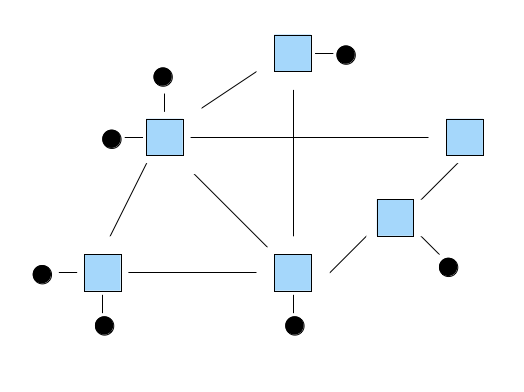
\includegraphics[width=.8\textwidth]{includes/network-model.png}
  \caption{Modèle de communication}
  \label{fig:commu}
\end{figure}

